\documentclass[12pt, titlepage]{article}

\usepackage{float}
\usepackage{geometry}
\usepackage{booktabs}
\usepackage{tabularx}
\usepackage{hyperref}
\usepackage{siunitx}
\hypersetup{
    colorlinks,
    citecolor=blue,
    filecolor=black,
    linkcolor=red,
    urlcolor=blue
}
\usepackage[round]{natbib}
\usepackage{amsmath, mathtools}
\usepackage{xr}
\externaldocument{../SRS/SRS}

\input{../Comments}
%% Common Parts

\newcommand{\progname}{Baja Dynamics} % PUT YOUR PROGRAM NAME HERE
\newcommand{\authname}{Team \#17, Team Name
\\ Grace McKenna
\\ Travis Wing
\\ Cameron Dunn
\\ Kai Arseneau} % AUTHOR NAMES                  

\usepackage{hyperref}
    \hypersetup{colorlinks=true, linkcolor=blue, citecolor=blue, filecolor=blue,
                urlcolor=blue, unicode=false}
    \urlstyle{same}
                                



\begin{document}

\title{System Verification and Validation Plan for \progname{}} 
\author{\authname}
\date{\today}
	
\maketitle

\pagenumbering{roman}

\section*{Revision History}

\begin{tabularx}{\textwidth}{p{3cm}p{2cm}X}
\toprule {\bf Date} & {\bf Version} & {\bf Notes}\\
\midrule
October 11th, 2024 & 0 & First version of VnV extra report\\
April 1st, 2025 & 1 & Added real-world data into VnV extra\\
\bottomrule
\end{tabularx}

~\\

\newpage

\tableofcontents

\listoftables


\listoffigures


\newpage

\section{Symbols, Abbreviations, and Acronyms}

\begin{table}[h]
  \raggedright
  \begin{tabular}{l l} 
    \toprule		
    \textbf{acronym} & \textbf{definition}\\
    \midrule
    CVT & Continuous Variable Transmission\\
    GPS & Global Positioning System\\
    IMU & Inertial Measurement Unit\\
    VnV & Verification and Validation\\
    \bottomrule
  \end{tabular}
  \caption{Verification and Validation Acronyms}
  \label{tab:vnv_acronyms}
\end{table}

\newpage

\pagenumbering{arabic}

\section{General Information}

\subsection{Summary}

\noindent This document will go into detail on the real-world data validation performed for the \progname{}. As per Dr. Smith's instructions, it will be completed prior to the course's end. This document currently serves as a placeholder for the final VnV extra report.

\section{Functional Tests Evaluation}

\subsection{Simulation Model}

\subsubsection{Position}

\begin{figure}[H]
  \begin{center}
   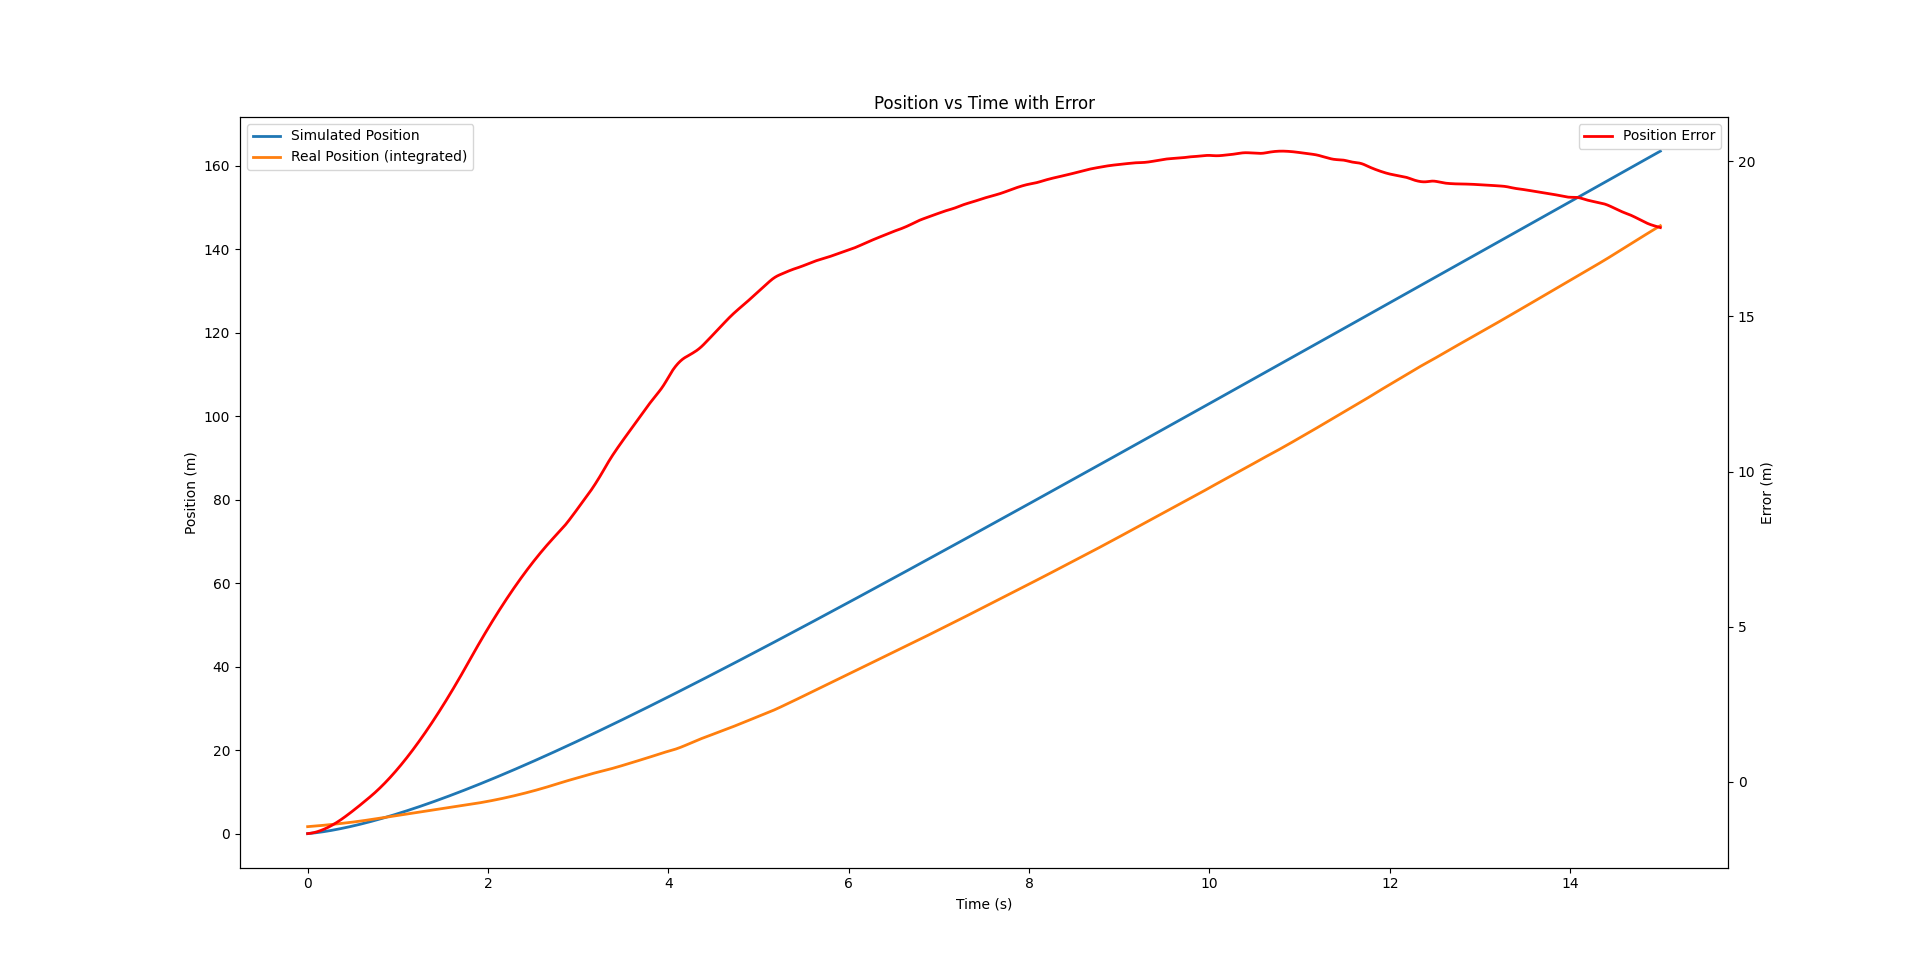
\includegraphics[width=\textwidth]{MSE Graphs/position.png}
  \caption{MSE of simulated position vs integrated experimental data.}
  \label{Fig_Position} 
  \end{center}
\end{figure}

- Car go fast... still! Explained by poor modelling of air resistance and other resistive forces such as rolling resistance, frictions, etc
- At the end you can see error decreases a bit. Perhaps the final force of air resistance was estimated too high, but the other forces were estimated too low, giving a slightly different final value, so final speed was too high.
- Also note the poor tests mentioned later about no max velocity

Car position over time

\subsubsection{Velocity}

\begin{figure}[H]
  \begin{center}
   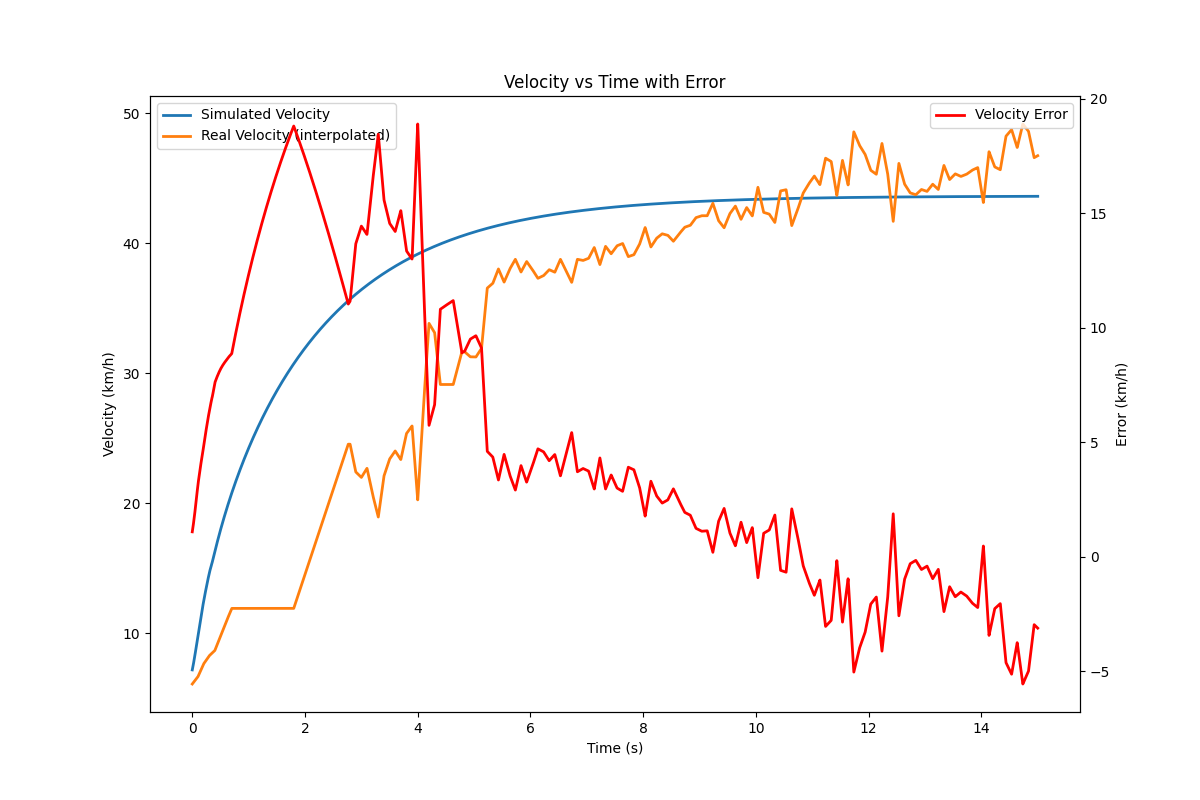
\includegraphics[width=\textwidth]{MSE Graphs/speed.png}
  \caption{MSE of simulated vehicle velocity and experimental data.}
  \label{Fig_Velocity} 
  \end{center}
\end{figure}

- Car go fast, shocker! Ignored many resistive forces, no slipping so early on its most noticeable.

Car velocity over time

\subsubsection{Acceleration}

Not availabel (no data gotten from IMU)

\subsubsection{Shift}

\subsubsection{Velocity}

\begin{figure}[H]
  \begin{center}
   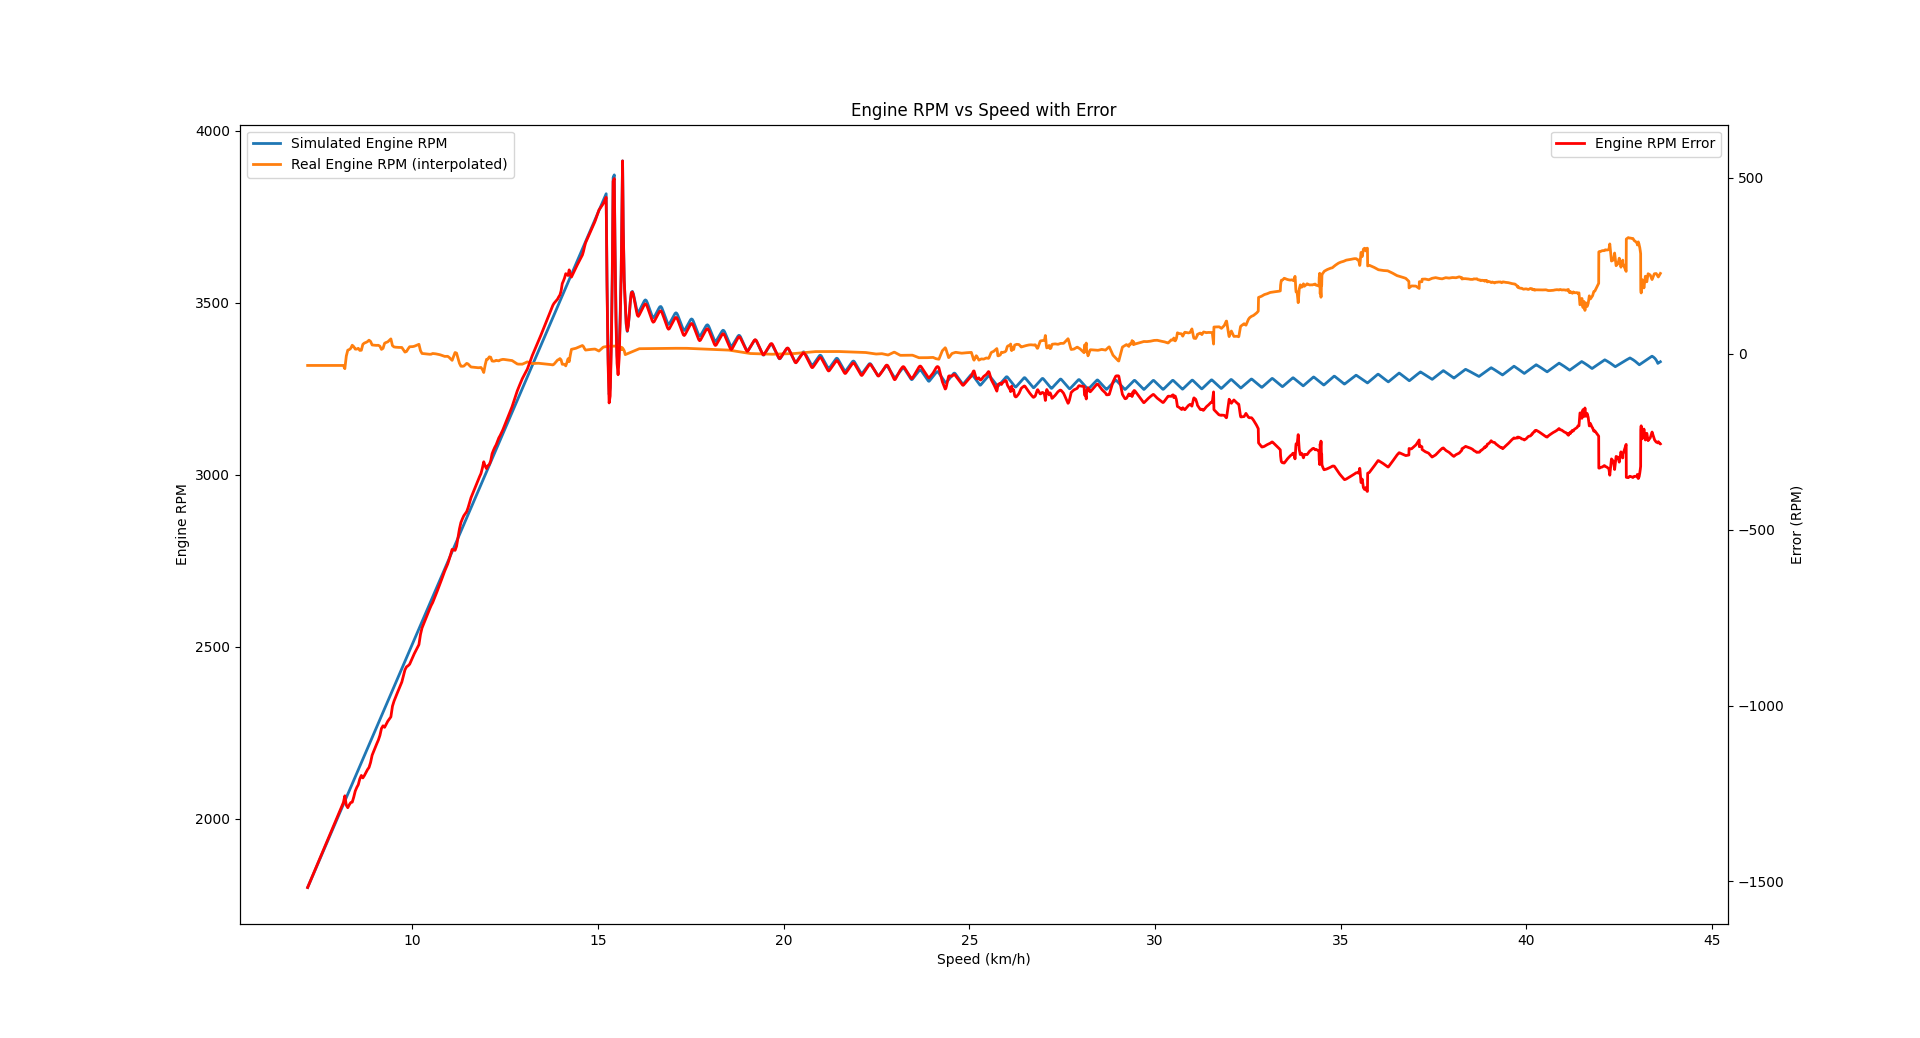
\includegraphics[width=\textwidth]{MSE Graphs/shift_curve_3400rpm.png}
  \caption{MSE of simulated shift curve and experimental data.}
  \label{Fig_Shift_3400} 
  \end{center}
\end{figure}

\begin{figure}[H]
  \begin{center}
   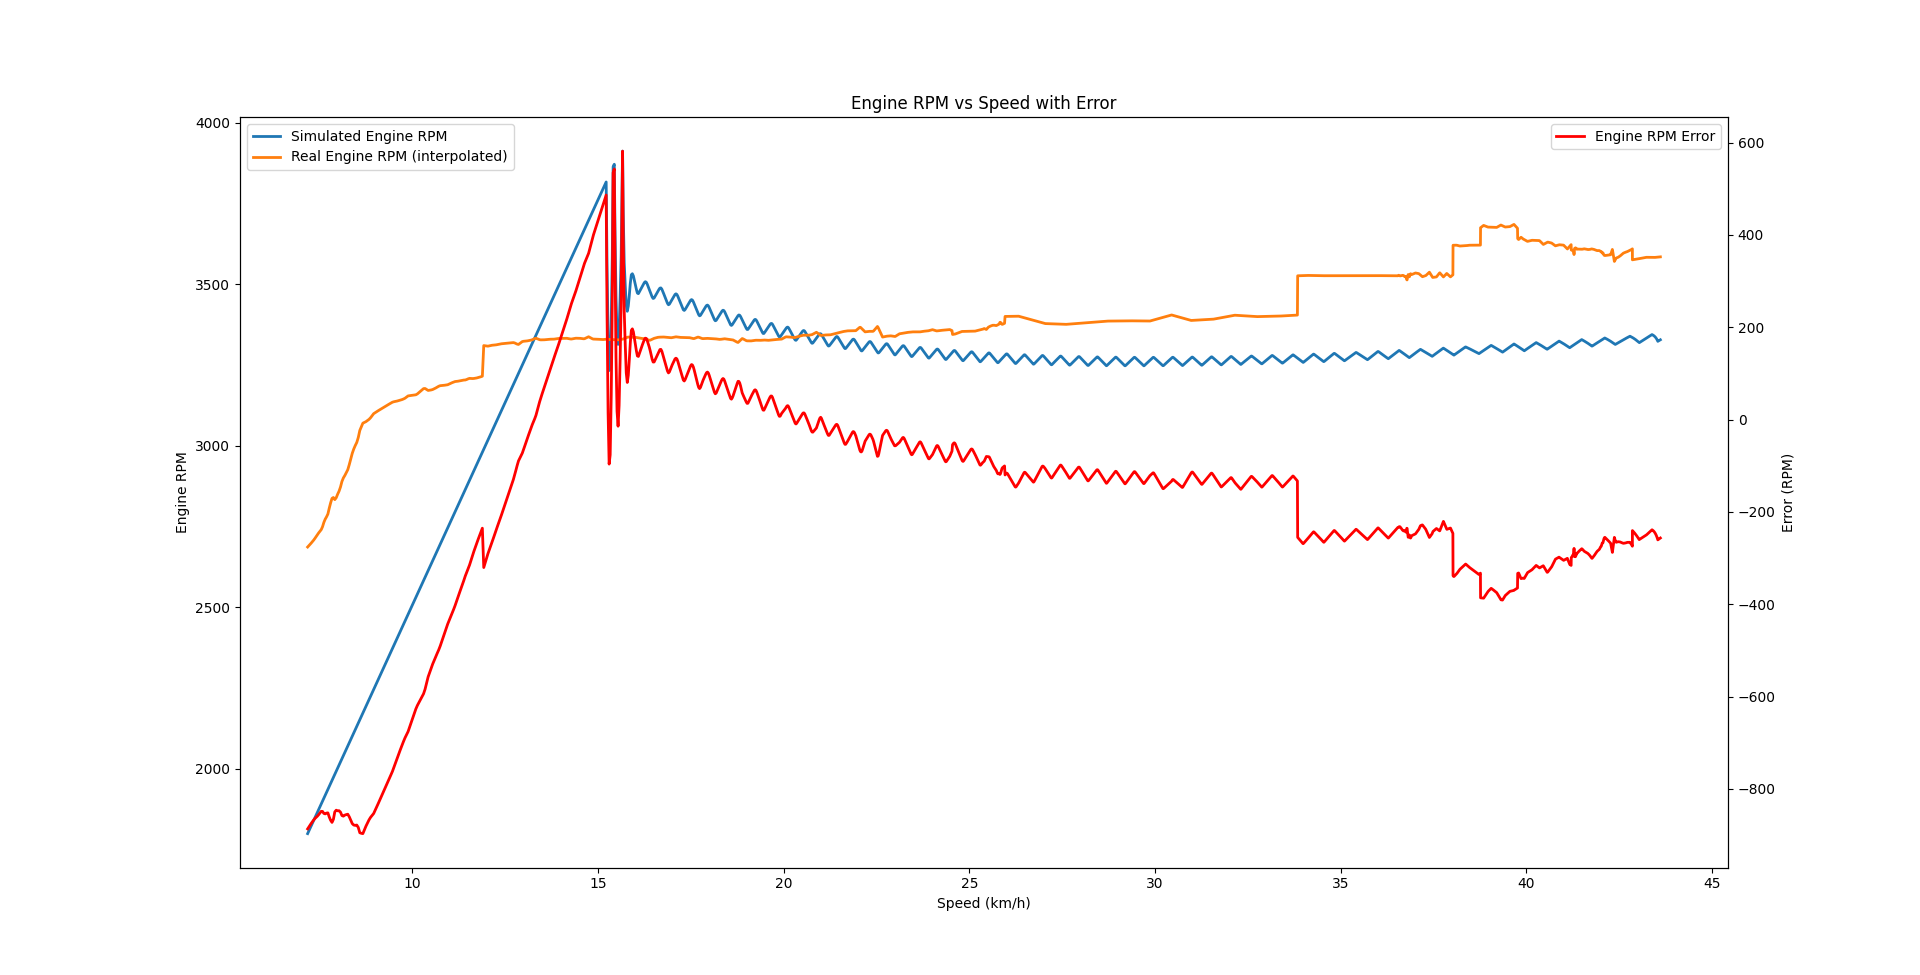
\includegraphics[width=\textwidth]{MSE Graphs/shift_curve_low_ratio.png}
  \caption{Second dataset at a different tune, showing the shift curve and experimental data.}
  \label{Fig_Shift_Low_Ratio} 
  \end{center}
\end{figure}

- We see generally a flat shift in both, which is great!
- Both also have a low ratio, although slight differences, they definitely both exist well

- Low ratio is somewhat different in calculations (causes: Wrong geometry, precision in machined parts, assumption of slip)
- Through the shift, we see some curve. A subtle change in ramps could cause this, or a poor understanding of the springs in our system. Potential in the real CVT system for spring to bind as it compresses, bringing unknown forces
- Don't see max shift much, this is due to poor data collection tests - Limits on the length of track we have access to mean we dont see our top end of the speeds our vehicle can acheive.


1 and 2 (What is 1?)

\section{Trace to Requirements or Modules}


\end{document}